\documentclass{beamer}
\beamertemplatenavigationsymbolsempty
\usecolortheme{beaver}
\setbeamertemplate{blocks}[rounded=true, shadow=true]
\setbeamertemplate{footline}[page number]
%
\usepackage[utf8]{inputenc}
\usepackage[english]{babel}
\usepackage{amssymb,amsfonts,amsmath,mathtext}
\usepackage{subfig}
\usepackage[all]{xy} % xy package for diagrams
\usepackage{array}
\usepackage{multicol}% many columns in slide
\usepackage{hyperref}% urls
\usepackage{hhline}%tables
% Your figures are here:
\graphicspath{ {fig/} {../fig/} }

%----------------------------------------------------------------------------------------------------------
\title{Using spatio-temporal dependencies to monitor additive manufacturing with deep learning}
\author[V.\,D.~Soldatov]{Vladislav Soldatov}
\institute{Moscow State University}
\date{\footnotesize
\par\smallskip\emph{Course:} My first scientific paper
\par\smallskip\emph{Expert:} 
\par\smallskip\emph{Consultant:} 
\par\bigskip\small 2023}

%----------------------------------------------------------------------------------------------------------
\begin{document}
%----------------------------------------------------------------------------------------------------------
% \begin{frame}
% \thispagestyle{empty}
% \maketitle
% \end{frame}
%-----------------------------------------------------------------------------------------------------
% \begin{frame}{Goal of research}
% ..
% \end{frame}
%-----------------------------------------------------------------------------------------------------
\begin{frame}{One-slide talk}

The use of additive manufacturing in industry is currently limited due to the unknown in advance and unreliable quality of parts.

\begin{columns}[c]
\column{0.6\textwidth}

\begin{figure}
    \centering
    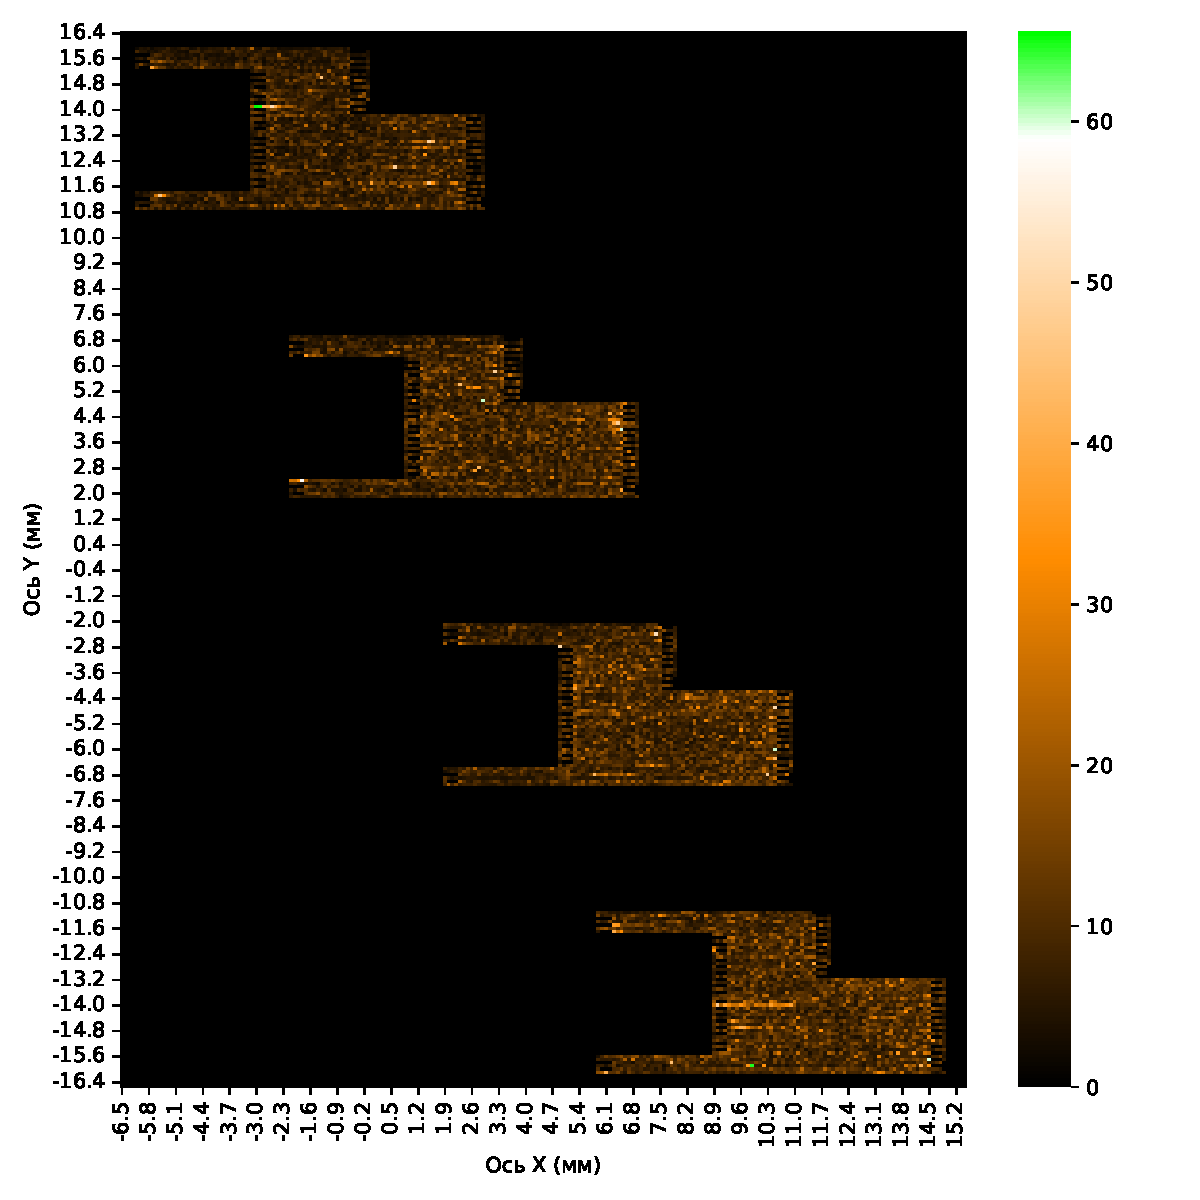
\includegraphics[scale=0.23]{lstm_4_window_xy_test_before.pdf}
    \caption{Coordinate distribution of the error function for the ConvLSTMAE model.}
    \label{fig:enter-label}
\end{figure}
\column{0.4\textwidth}
    \textbf{Main task:} detect anomalous situations in AM processes on-line.

    \textbf{Specifics:} given a sequence of meltpool frames, predict if laser will stumble across an obstacle at a certain point in time.
    
    %  This is largely caused by complex relationships between process parameters. Therefore, it is important to develop methods for monitoring AM processes in real time to ensure the quality of parts.

\end{columns}

% \bigskip
{\footnotesize {\color{red} Tags:} Additive manufacturing $\cdot{}$ Laser Powder Bed Fusion $\cdot{}$ Online monitoring $\cdot{}$ Flaw detection $\cdot{}$ Porosity prediction $\cdot{}$ Spatial-temporal Modeling}
\end{frame}


%----------------------------------------------------------------------------------------------------------
% \begin{frame}{Problem statement}
% ..
% \end{frame}
%----------------------------------------------------------------------------------------------------------
% \begin{frame}{Solution}
% \begin{columns}[c]
% \column{0.6\textwidth}
%     Column 1
% \column{0.4\textwidth}
%     Column 2
% \end{columns}
% \end{frame}
%----------------------------------------------------------------------------------------------------------
% \begin{frame}{Computational experiment}
% ..
% \end{frame}
%----------------------------------------------------------------------------------------------------------
% \begin{frame}{Conclusion}
%     \begin{block}{Forecast with hierarchical aggregation of}
%     \begin{itemize}
%         \item types of freight in
%         \item stations, regions, and roads,
%         \item for a day, week, month, and quarter.
%     \end{itemize}
%     \end{block}
% \end{frame}
%----------------------------------------------------------------------------------------------------------
\end{document} 